\documentclass[a4paper, 14pt]{article}

\usepackage[english, russian]{babel}
\usepackage[T2A]{fontenc}
\usepackage[utf8]{inputenc}
\usepackage{indentfirst}





\frenchspacing   
\usepackage{amsmath,amsfonts,amssymb,amsthm,mathtools}
\usepackage{graphicx} % for reflect boc
 % пакеты AMS
\usepackage[hidelinks]{hyperref}

\usepackage{icomma}                                    % "Умная" запятая
\usepackage{NiceMatrix}

\usepackage{physics}
\usepackage{slashed}
\usepackage{tikz}
\usepackage{feynmp}
\usepackage{tikz-feynman}
\usepackage{pgfplots}
\pgfplotsset{compat=newest}

\usepackage{geometry}
\geometry{top=25mm}
\geometry{bottom=30mm}
\geometry{left=20mm}
\geometry{right=20mm}

\linespread{1}

%Колонтитулы
\usepackage{titleps}
\newpagestyle{main}{
	\setheadrule{0.4pt}
	\setfootrule{0.4pt}
	\setfoot{}{\thepage}{}
}
\pagestyle{main}
\newcommand{\deriv}[2]{\frac{\partial #1}{\partial #2}}
\newcommand{\cderiv}[2]{\cfrac{\partial #1}{\partial #2}}
\newcommand*{\Eval}[3]{\left.#1\right\rvert_{#2}^{#3}}

\newcommand{\fderiv}[2]{\frac{d #1}{d #2}}
\newcommand{\tderiv}[1]{\frac{d #1}{d t}}

\newcommand{\cfderiv}[2]{\cfrac{d #1}{d #2}}
\newcommand{\ctderiv}[1]{\cfrac{d #1}{d t}}

\newcommand{\sn}[2]{\ensuremath{{#1}\cdot 10^{#2}}}

\newcommand{\dxv}[1]{d^3 {#1}}
\newcommand{\dpv}[1]{\cfrac{d^3 {#1}}{(2\pi)^3}}

\newcommand{\lvec}[1]{\reflectbox{\ensuremath{\vec{\reflectbox{\ensuremath{#1}}}}}}

\newcommand{\avarage}[1]{\left\langle #1 \right\rangle}
\begin{document}
	
	\tableofcontents
	\section{Introduction}
	Наличие тёмной материи – это хорошо хорошо установленный факт, следующий из астрофизических наблюдений и космологических данных. Тёмная материя составляет основную массу галактик, объясняя форму кривой вращения, входит в уравнения Фридмана эволюции Вселенной а также играет ключевую роль в образовании крупномасштабной структуры Вселенной. 	Тёмная материя практически не взаимодействует с веществом, поэтому состав тёмной материи неизвестен. Вероятно, что она состоит из новых частиц вне Стандартной модели физики частиц. Одним из классов таких частиц являются слабовзаимодействующие массивные частицы (WIMPs), которые мы будем рассматривать.


Образование частиц тёмной материи объясняется механизмом freeze-out, при котором частицы находились в термальном равновесии с  плазмой, о потом вышли из равновесия вследствие расширения Вселенной. Для объяснения плотности тёмной материи $\Omega h^2 = 0.12$ необходимо, чтобы сечение аннигиляции тёмной материи в частицы стандартной модели имело порядок $10^-26 \text{см}^3/\text{c}$. Сечения такого порядка характерны для процессов электрослабого масштаба. В таком случае эти частицы можно зарегистрировать различными способами. Наиболее чувствительным методом является прямое детектирование частиц в галактическом гало путём измерения отдачи ядер в низкофоновых экспериментах, таких как XENON, PANDAX. Отсутствие сигнала накладывает сильные ограничения на упругое сечение взаимодействия с нуклоном $\sigma_{\chi n}$ (рисунок).


Однако эти ограничения могут быть ослаблены, если тёмная материя является неупругой: частицам в гало не будет хватать энергии для преодоления порога реакции рассеяния на ядре. Тогда более чувствительным методом поиска тёмной материи может стать детектирование нейтрино от аннигиляции тёмной материи захваченной и накопленной внутри Солнца. Для того, чтобы дать предсказание потоков нейтрино нужно найти скорость захвата частиц тёмной материи $C$, распределение этих частиц на текущий момент и темп аннигиляции. Имея темп аннигиляции можно найти спектр нейтрино. В случае упругой тёмной материи частицы быстро термализуются и имеют распределение Больцмана с температурой близкой к температуре в центре Солнца. Для исследуемой области параметров масса - сечение $m_{\chi} - \sigma{\chi p}$ это означает, что темп аннигиляции в текущий момент должен совпадать с темпом захвата. Однако как было показано в работе [1], неупругая тёмная материя в какой-то момент времени перестанет термализоваться из-за энергетического порога. В таком случае темп аннигиляции может быть существенно меньше темпа захвата, что уменьшит чувствительность метода и, значит, ослабит ограничения.


В данной работе мы пересмотрим численное решение термализации тёмной материи в Солнце и найдём соотношение между аннигиляцией и захватом а также найдём область параметров тёмной материи, при которой равновесие между аннигиляцией и захватом всё ещё наступает.
	
	\section{Inelastic Dark Matter in the Sun}
	Для того, чтобы была аннигиляция тёмной материи в Солнце, она должна накопиться в достаточном количестве. Количество частиц, захваченное из гало за единицу времени обозначают как $C$. Темп аннигилляции $A$ зависит от количества частиц $N$ и их распределения. Темп захвата равен $aN^2$, где $a$ --- зависит только от распределения частиц. 

Уравнение на полное число частиц выглядит следующим образом:

\begin{equation}
	\label{eq:Balance}
	\tderiv{N} = C - aN^2
\end{equation}

\noindent и имеет решение в момент времени $t$:
\begin{equation}
\begin{split}
	N = \sqrt{\cfrac{C}{a}} \th{[\sqrt{aC}t]} \\
	A = aN^2 = C \th^2{[\sqrt{at^2C}]}
	\label{eq:AnnNtherm}
\end{split}
\end{equation}
	

В случае упругой тёмной материи коэффициент $a$ определяется термальным распределением:
\begin{equation}
	a_{el} = \cfrac{
		\avarage{\sigma_{a}v} \int{d^3 r e^{-2 \frac{m_{\chi}\phi(r)}{T_{\chi}} }}
	}{\left(
		\int{d^3 r e^{- \frac{m_{\chi}\phi(r)}{T_{\chi}} }}
	\right)^2}
\end{equation}

В случае, когда масса тёмной материи больше $10$ GeV, температуру термального распределения $T_{\chi}$ можно взять равной температуре в центре Солнца $T_{\odot}(r=0) = 1.33\cdot10^{-6} \text{GeV}$, а потенциал $\phi(r)$ разложить до квадратичного порядка: $\phi(r) =\phi(0)+ \frac{v_{esc}^2}{2} \frac{\rho_0}{2} \frac{r^2}{R_{\odot}^2} + o(r^2)$,  где $\rho_0 = 105.7$. Тогда

\begin{equation}
	a_{el} = \cfrac{1}{(4\pi)^{3/2}} \cfrac{\avarage{\sigma_{a}v}}{ r_{\chi}^3 }
\end{equation}

где

\begin{equation}
	r_{\chi} = R_{\odot} \sqrt{\cfrac{2 T_{\odot}(0) }{m_{\chi}\rho_0 v_{esc}^2}} =  0.077 R_{\odot} \sqrt{\cfrac{ \text{GeV}}{m_{\chi}}}
\end{equation}

Приведём значение для $a_{el}t^2$ в момент возраста Солнца $T_{\odot}$

\begin{equation}
	a_{el}T_{\odot}^2 = 
	9\cdot10^{-23} \text{s}	\left(\cfrac{   \avarage{\sigma_{a}v}    }{3\cdot10^{-26} \text{cm}^2\text{s}^{-1}} \right)
	\left(\cfrac{m_{\chi}}{\text{GeV}}\right)^{3/2}
\end{equation}

Для неупругого случая, уравнения эволюции хоть и не учитывают распределение частиц, но всё равно оказываются верными в переходной области, где $C$ и $A$ имеют схожее значение. 
В неупругом случае этот зависит от массы тёмной материи $m_{\chi}$, разницей масс основного и возбуждеённого состояния $\delta$ и от сечения аннигиляции $\avarage{\sigma_{a}v}$ (мы брали $\avarage{\sigma_{a}v} = 3\cdot 10^{-26} \text{cm}^3/\text{s}$). Поэтому для нахождения темпа аннигиляции нужно воспользоваться формулой выше и наёденными численно коэффицентами $a$.
	\subsection{Capture}
	

Захват тёмной материи происходит следующим образом. Изначально тёмная материя находится в гало (вдали от Солнца) и имеет некоторое распределение по скоростям $f(u)$. Затем она попадает в Солнце, где может столкнуться с ядрами вещества, потеряв часть кинетической энергии. Частица будет захвачена, если её финальная скорость будет меньше скорости вылета в точке столкновения $v’ < v_{esc}(r)$. Таким образом, величина захвата – это сумма по всем ядрам мишеням темпа столкновений тёмной материи:

\begin{equation}
	\label{eq:Capture_Full}
	C = \sum_{\alpha} C_{\alpha} = \sum_{\alpha} \int{
		d^3\vec{x} \cdot d^3\vec{v} \cdot f(v^2,r) \cdot n_{\alpha}(r) 
		d^3\vec{v}_{\alpha} f_B(v_{\alpha},T(r)) \cdot
		|\vec{v}- \vec{v}_{\alpha}| d\sigma_{\chi \alpha}
	}
\end{equation}

где $v$ --- скорость тёмной материи в точке $r$, $n_{\alpha}(r)$ --- концентрация ядер сорта $\alpha$, $f_B(v_{\alpha},T(r))$ --- Больцмановское распределение по скоростям ядер с локальной температурой $T(r)$, $d\sigma_{\chi \alpha}$ --- дифференциальное сечение тёмной материи и ядра. Интеграл по дифференциальному сечению идёт по области, когда $v’ < v_{esc}(r)$

Мы представим $C_{\alpha}$ следующим образом:

\begin{equation}
	\label{eq:Capture_a}
	C_{\alpha} = V_{\odot} n_{\chi 0.4} \cdot
	\sigma_{\chi p} n_{p} v_{esc} \cdot c_{\alpha} = 
	\cfrac{N_{\odot}}{T_{\chi p}} \cdot c_{\alpha}
\end{equation}

Где $V_{\odot}$ --- полный объем Солнца, $n_{\chi 0.4}$ --- локальная концентрация частиц тёмной материи ($0.4 \text{GeV}/\text{cm}^{3}$), $\sigma_{\chi p}$ --- характерное сечение взаимодействия тёмной материи и ядра, $v_{esc} = v_{esc}(r = R_{\odot})$ --- скорость вылета тёмной материи на краю Солнца. Мы определили $N_{\odot} = V_{\odot} n_{\chi 0.4} = 5.64\cdot10^{32} \frac{\text{GeV}}{m_{\chi}}$, а $T_{\chi p} = (\sigma_{\chi p} n_{p} v_{esc})^{-1}$, что равно $1.92\cdot 10^{10} \text{s}$.

Тогда 

\begin{equation}
	\label{eq:ca_coeff}
	c_{\alpha} = \int  \left[3r^2 dr  \right] \cdot \left[4\pi v \cdot u d u \cdot f_{eff}(u)  \right]  \cdot 
	\left[ \rho(r)\cfrac{\tilde{\rho}_{\alpha}(r)}{A_{\alpha}}  \cdot f_B(v_{\alpha}) d^3 \vec{v}_{\alpha} 
	\right] \cdot F(q,v) \cfrac{v'}{v_{esc}} \cdot \cfrac{d \Omega}{4\pi} 
\end{equation}

где: $r$ обозначает безразмерный радиус, меняющийся от $0$ до $1$, $\rho(r)$ --- плотность вещества, нормированная согласно $\int \rho(r) 3r^2 dr = 1$, $\tilde{\rho}_{\alpha}(r)$ --- массовая доля элемента $\alpha$ в точке $r$, $A_{\alpha}$ --- число нуклонов в ядре, $v'$ --- разность скоростей тёмной материи и ядра после столкновения. $f_{eff}(u)$ --- распределение частиц тёмной материи вдали от Солнца с учётом движения солнца со скоростью $u_0$ (скорость тёмной материи вдали Солнца $u$ и скорость $v$ в точке $r$ связанны соотношением $v^2 = u^2 + v_{esc}^2(r)$)

\begin{equation}
	f_e(u^2) = \int_{-1}^1 {f(u^2+u^2_0 + 2 u u_0 \cos{\theta}) \cfrac{d\cos{\theta}}{2}}
\end{equation}

В качестве распределения вдали от Солнца возьмём распределение Максвелла, ограниченное максимальной скоростью $u_{max}$

\begin{equation}
	f(u)  = \cfrac{1}{(2\pi \xi^2)^{3/2}} e^{-\frac{u^2}{2 \xi^2}} \cdot \theta(u_{max} - u )
\end{equation}

Мы предполагаем следующие параметры (из стандартной модели гало):
$v_{esc} = 2.06 \cdot 10^{-3} = 618 \frac{\text{km}}{\text{s}}$, $\xi = 0.423 \cdot 10^{-3} = 127 \frac{\text{km}}{\text{s}}$, $u_0 = 0.733 \cdot 10^{-3} = 220 \frac{\text{km}}{\text{s}}$, $u_{max} = 1.78 \cdot 10^{-3} = 533 \frac{\text{km}}{\text{s}}$.

$F(q,v)$ --- это форм фактор ядра, определённый следующим образом:

\begin{equation}
	\label{eq::ff_def}
	F(q,v) = \cfrac{(m_{\chi} + m_{p})^2}{(m_{\chi} + m_{\alpha})^2}
	\cfrac{|\mathcal{M}_{\chi \alpha}|^2}
	{|\mathcal{M}_{\chi p}|^2}
\end{equation}

где $|\mathcal{M}_{\chi \alpha}|^2$ --- усреднённый по спинам матричный элемент рассеяния тёмной материи на ядре, а $|\mathcal{M}_{\chi p}|^2$ --- на нуклоне.

Величину $\sigma_{\chi p}$ мы определяем как:

\begin{equation}
	\label{eq:sigma_def}
	\sigma_{\chi p} = \int {\cfrac{|\mathcal{M}_{\chi p}|^2}{64\pi^2 (m_{\chi} + m_p)^2} d\Omega}
\end{equation}




	\subsection{Thermalization}
	Когда тёмная материя захватывается, она далее испытывает вторичные столкновения с веществом и аннигиляцию. Её эволюция описывается уравнением Больцмана на функцию распределения $f(\vec{r},\vec{v})$:

\begin{equation}
	\label{eq:Boltsman}
	\deriv{f}{t}(\vec{r},\vec{v}) + \vec{v} \deriv{f}{\vec{r}}(\vec{r},\vec{v}) - \nabla \phi \deriv{f}{\vec{v}}(\vec{r},\vec{v}) = 
	St[f] (\vec{r},\vec{v})
\end{equation} 
где $St[f]$ --- интеграл столкновений. Этот член значительно меньше левой части уравнения (что следует из того, что длина свободного пробега частицы $\chi$ значительно превышает размер Солнца). Следовательно, для решения этого уравнения нужно перейти из пространства $\vec{r}-\vec{v}$ в пространство $E-L$, где $E$ --- энергия тёмной материи, а $L$ --- момент импульса. Линейная часть уравнение Больцмана, связанная с рассеяниям на ядрах, имеет вид:

\begin{equation}
	\label{eq:BoltsmanEL}
	\deriv{f}{t}(E,L) = C(E,L) + \int{ S(E_i,L_i,E,L) f(E_i,L_i) dE_idL_i } 
	-f(E,L) \int{ S(E,L,E_f,L_f)  dE_fdL_f }
\end{equation}

В уравнение входят также член, отвечающий за аннигиляцию, и член, отвечающий за рассеяние частиц тёмной материи на самой себе, который в данной работе считается малым по сравнениею с аннигиляцией и не учитывается.

Для учёта аннигиляции в (\ref{eq:BoltsmanEL}) добавляется 
\begin{equation}
	-\label{eq:BoltsmanAnn}
	f(E,L) \int{ A(E,L,E',L') f(E',L') dE'dL' }
\end{equation}

Для удобства, мы используем безразмерные величины энергии $E$ и момента импульса $L$, которые определены следующим образом:
\begin{equation}
	\begin{split}
		E = \cfrac{\frac{1}{2} v_{\chi}^2 + \phi(r)}
		{\frac{1}{2} v_{esc}^2} \\
		L = \cfrac{|\vec{r} \times \vec{v}|}
		{R_{\odot} v_{esc}}
	\end{split}
	\label{eq:dimentionless}
\end{equation}

Еще одна величина --- приведенный момент импульса.
\begin{equation}
	l = \cfrac{L}{L_{max}(E)}
\end{equation}

где $L_{max}(E)$ --- максимально возможный момент импулься траектории при данной энергии (при этом не учитываются траектории, которые находятся вне Солнца).



Для численного решения уравнения мы разбиваем пространство на прямоугольные бины по величинам энергии $E$ и приведенного момента $l$. Внутри бина мы считаем, что частицы распределены относительно какой-то меры: это может быть $d\Phi = dEdL$ либо $d\Phi = dEdL^2$ (мы используем второй вариант). 

Eравнение эволюции на число частиц $N_{i}$ в бине $i$ будет иметь вид:

\begin{equation}
	\label{eq:evolution}
	\deriv{N_{i}}{t} = \cfrac{1}{T_{\chi p}} \left(N_{\odot} c_i +
	\sum_j{[s_{ij} N_{j} - s_{ji} N_{i} ]} - e_{i} N_i - \cfrac{a_{\gamma}}{N_{\odot}} \sum_j {a_{ij} N_j N_i} \right)
\end{equation}

Величины $c_i$ определяются из интеграла (\ref{eq:ca_coeff}), но интеграл ограничивается областью, в которой конечные $E$ и $L$ частицы попадают в бин $i$.
Величины $s_{ij}$ определяют вероятности переёти из бина $j$ в бин $i$ и вычисляются аналогично $c_{i}$. Как $c_{i}$ так  $s_{ij}$ мы вычисляем методом Монте-Карло.

\begin{equation}
	\label{eq:st_integral}
	s_{ij} = \sum_{\alpha}\int{
		\cfrac{d\Phi_{j}}{\mu(\Phi_{j})}
		\cfrac{T_{in}(\Phi_{j})}{
			T_{in}(\Phi_{j})+T_{out}(\Phi_{j})
		} \cdot d\tau \left[ f_B(v_{\alpha}) d^3 \vec{v}_{\alpha} \right] \cdot \cfrac{v'}{v_{esc}} F(q,v) \cfrac{d\Omega}{4\pi}
	}
\end{equation}

\noindent Интеграл $d\Phi_{j}$ обозначает интегрирование по фазовому объёму бина $j$, причём $\mu(\Phi_{j}) = \int{d\Phi_{j}}$ равен $1$. В выражении присутствует интегрирование вдоль траектории движения частицы в потенциале $\phi(r)$. Величина $\tau$ параметризует внутреннюю части траектории и пробегает от $0$ до $1$. $T_{in} + T_{out}$ --- время, за которое частицы проходит от минимального $r_{min}$ до максимального $r_{max}$ положения. Это время разбивается на время пребывания внутри Солнца $T_{in}$ и Снаружи $T_{out}$. Мы используем также обезразмеренное время на $R_{\odot}/v_{esc}$.

\begin{equation*}
	T(E,L) = \int_{r_{min}}^{r_{max}}{\cfrac{dr}{
			\sqrt{E - \varphi(r) - \frac{L^2}{r^2}}
		} 
	}
\end{equation*}

где $\varphi(r)$ --- определяет Ньютоновский потенциал:

\begin{equation*}
	\phi(r) = \cfrac{GM(r)}{r} = \varphi(r) \cfrac{v_{esc}^2}{2} 
\end{equation*}

$\varphi(r)$ удовлетворяет уравнению Пуассона:

\begin{equation}
	\cfrac{1}{r^2}\deriv{}{r}
	\left(r^2\deriv{\varphi(r)}{r}\right) = 3\rho(r)
\end{equation}

где $\rho(r)$ --- отношение плотности к средней плотности из (\ref{eq:ca_coeff}).


Те частицы, которые не попали ни в какой бин $i$ в интеграле (\ref{eq:st_integral}) испаряются, что определяет величину $e_i$, т.е. $e_i$ = $s_{i'i}$, где $i'$ --- формальный индекс бина: $(E,l) \in [0,+\infty]\times[0,1]$.

Коэффициент $a_{\gamma}$ определяет соотношения скорости аннигиляции и столкновений и равен:

\begin{equation}
	a_{\gamma} = \cfrac{ \avarage{\sigma_{\chi\chi} v} n_{\chi 0.4}}{\sigma_{\chi p} n_{p} v_{esc}} = 
	T_{\chi p} \cdot \avarage{\sigma_{\chi\chi} v} n_{\chi 0.4}
\end{equation}
где $\avarage{\sigma_{\chi\chi} v}$ --- произведение сечения аннигиляции на скорость, которое мы брали равным $3\cdot10^{-26}\text{cm}^3\,{s^{-1}}$. Тогда $a_{\gamma} = 2.31\cdot10^{-16} \frac{\text{GeV}}{m_{\chi}}$. Выражения для $a_{ij}$ мы приведём в аппендиксе.


	%\subsection{Annihilation}
	
	\section{Scenarious}
	В формулах для рассеяния выше фигурировал формфактор $F(q,v)$ (\ref{eq::ff_def}). Его значение является модельно зависимым. Для определения формфактора в конкретных моделях находится из релятивисткой теории нерелятивисткий оператор $\hat{V}$ взаимодействия частиц тёмной материи и нуклонов.
$\hat{V}$ раскладывается на линейную комбинацию операторов $\hat{O}_i$.
\begin{equation}
	\hat{V}_{\chi N}(\vec{r}_{\chi} - \vec{r}_{N}) = \sum_i{c_i \hat{O}_i} 
\end{equation}
А гамильтониан взаимодействия тёмной материи и ядра является суммой $\hat{V}_{\chi N}$ по всем нуклонам:
\begin{equation}
	\mathcal{H}_{int} = \sum_{k}{\hat{V}_{\chi k}(\vec{r}_{\chi} - \vec{r}_{k})} 
\end{equation}

Вычисление матричных элементов от $\mathcal{H}_{int}$ рассматривается в работах [refs]. 

В случае упругой тёмной материи рассматривают 2 сценария: когда взаимодействие является спин-независимым и спин зависимым. 
Например, многих моделях фермионной тёмной материи, взаимодействие с нуклонами имеет вид $\bar{\chi}\gamma^{\mu}\chi \bar{N}\gamma^{\mu}N$, что соответствует спин независимому оператору $\hat{O}_1 = 1$ или $\bar{\chi}\gamma^{\mu}\gamma^{\mu}\chi \bar{N}\gamma^{\mu}\gamma^{5}N$, что соответствует спин зависимому оператору $-4\hat{O}_4 = -4c \vec{S}_{\chi}\cdot\vec{S}_{N}$.

Неупругая тёмная материя возникает в достаточно специфичных сценариях. В данной работе мы рассмотрим неупругую тёмную материю со спин независимым взаимодействием с нуклоном $c \hat{O}_1$ а также тёмную материю c магнитным моментом $\mu_{\chi}$ со следующим взаимодеёствием с электромагнитным полем:
	\begin{equation*}
	\mathcal{L}_{int} = \cfrac{\mu_{\chi}}{2} \bar{\Psi}_1 \Sigma_{\mu\nu} \Psi_2 F^{\mu\nu} + \cfrac{\mu_{\chi}}{2} \bar{\Psi}_2 \Sigma_{\mu\nu} \Psi_1 F^{\mu\nu} 
\end{equation*}
где ${\Psi}_{1,2}$ --- майорановские спиноры, состояний $1$ и $2$, а $\Sigma_{\mu\nu} = \frac{i}{2}[\gamma_{\mu}\gamma_{\nu}]$.

Нерелятивисткий опреатор взаимодействия с нуклоном тогда следующий:
\begin{equation}
	\mathcal{H} = 
	\cfrac{Q_N e\mu_{\chi}}{2m_{\chi}} \hat{O}_1 + 
	\cfrac{2g_N e\mu_{\chi}}{m_{N}} \hat{O}_4-
	\cfrac{2Q_N e\mu_{\chi} m_{N} }{q^2} \hat{O}_5 -
	\cfrac{2g_N e\mu_{\chi} m_{N}}{q^2} \hat{O}_6
\end{equation}

где $e Q_N$ --- заряд нуклона,  $g_N$ --- множитель Ланде нуклона.


\begin{eqnarray}
	\hat{O}_1 = 1 & 
	\hat{O}_4 = \vec{S}_{\chi}\cdot\vec{S}_{N} \\
	%
	\hat{O}_5 = i\vec{S}_{\chi}\cdot \left(\cfrac{\vec{q}}{m_N} \times \vec{v}^{\perp}_{inel} \right) & 
	\hat{O}_6 = \left(\vec{S}_{\chi} \cdot \frac{\vec{q}}{m_N}\right)\left(\vec{S}_N \cdot \frac{\vec{q}}{m_N}\right)
\end{eqnarray}

где $\vec{q} = \vec{k} - \vec{k}'$ --- переданный импульс от тёмной материи к веществу, а 
\begin{equation}
	\vec{v}^{\perp}_{inel} = \vec{v}^{\perp}_{el} + \cfrac{\delta}{q^2} \vec{q} = \vec{v}+\cfrac{\vec{q}}{2\mu_{N}} + \cfrac{\delta}{q^2} \vec{q}
\end{equation}

	
	
	
	\section{Numerical Results}
	%
	% 	 1) Картинки с захватом и распределением по E,L
%		вначале и в конце эволюции (100 GeV, 100 KeV)
%	 2) Картинки для Скорости захвата и аннигиляции 
%		C(delta) и A(delta) с учётом аннигиляции и без %		учёта аннигиляции, сравнение с tan^2()
%	 3) Коэффициент аннигиляции a как функция от delta %		и m
%	 4) Графики в плоскости M,delta где есть равновесие	
%    
В нащем численном моделировании мы использовали неравномерную решетку: интервал по $l$ мы разбивали на $90$ равных частей, а по $E$ мы увеличивали плотность разбиения при мальеньких $E$.

Изобразим распределение частиц по энергии и моменту импульса (на единицу массы частицы). 

Мы будем рассматривать распределение частиц по энергтт и приведеному импульсу $f(E,l) = \frac{dN}{dE dl}$.

\begin{figure}[ht]
	\centering
	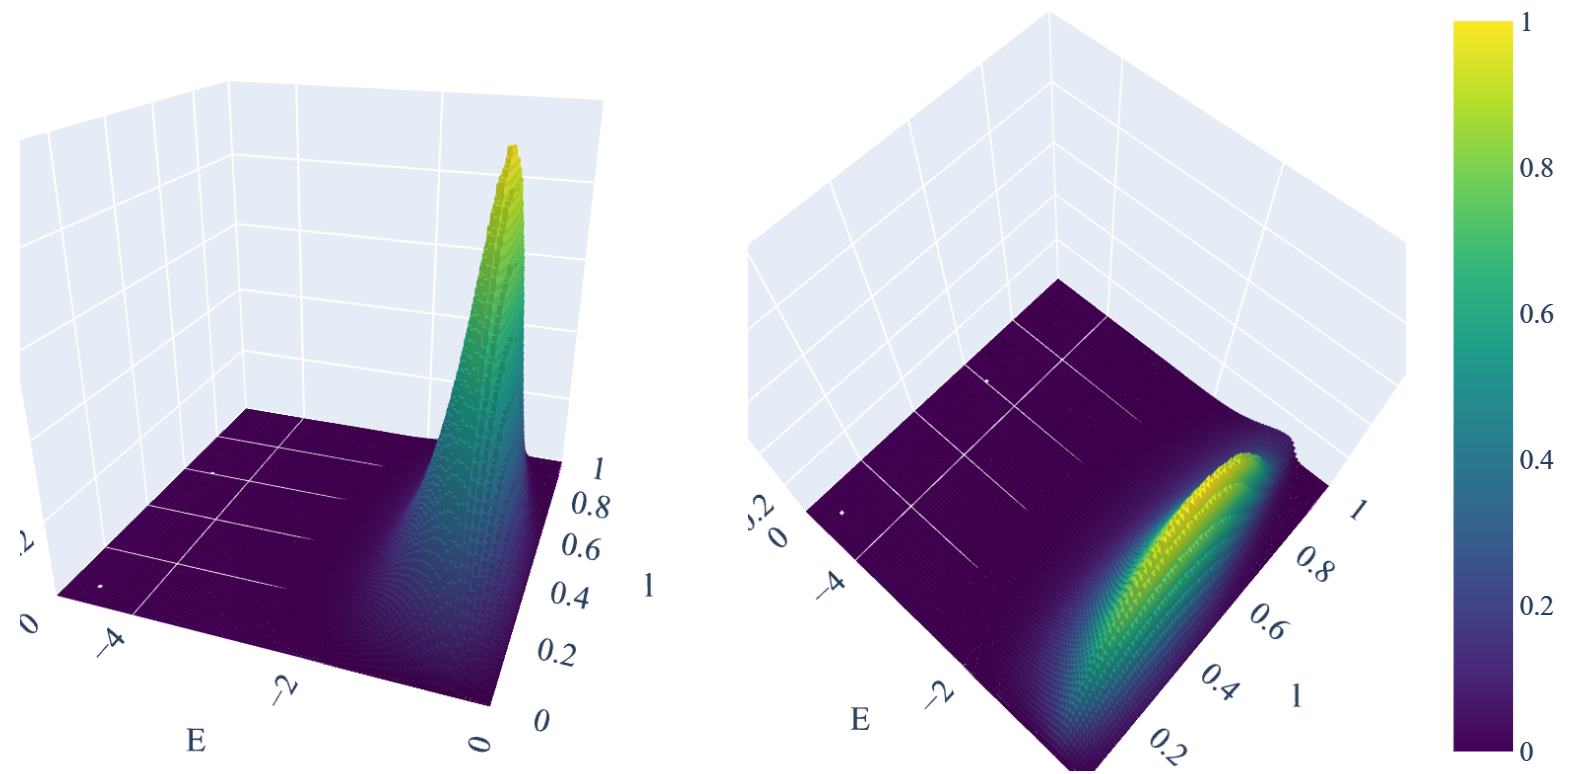
\includegraphics[width=0.7\textwidth]
	{images/Capt100_100.png}
	\caption{Распределение захваченных частиц для $m_{\chi} = 100\, \text{GeV}$, $\delta = 100\, \text{keV}$.}
	\label{fig:Capt100_100}
\end{figure}

\begin{figure}[!h]
	\centering
	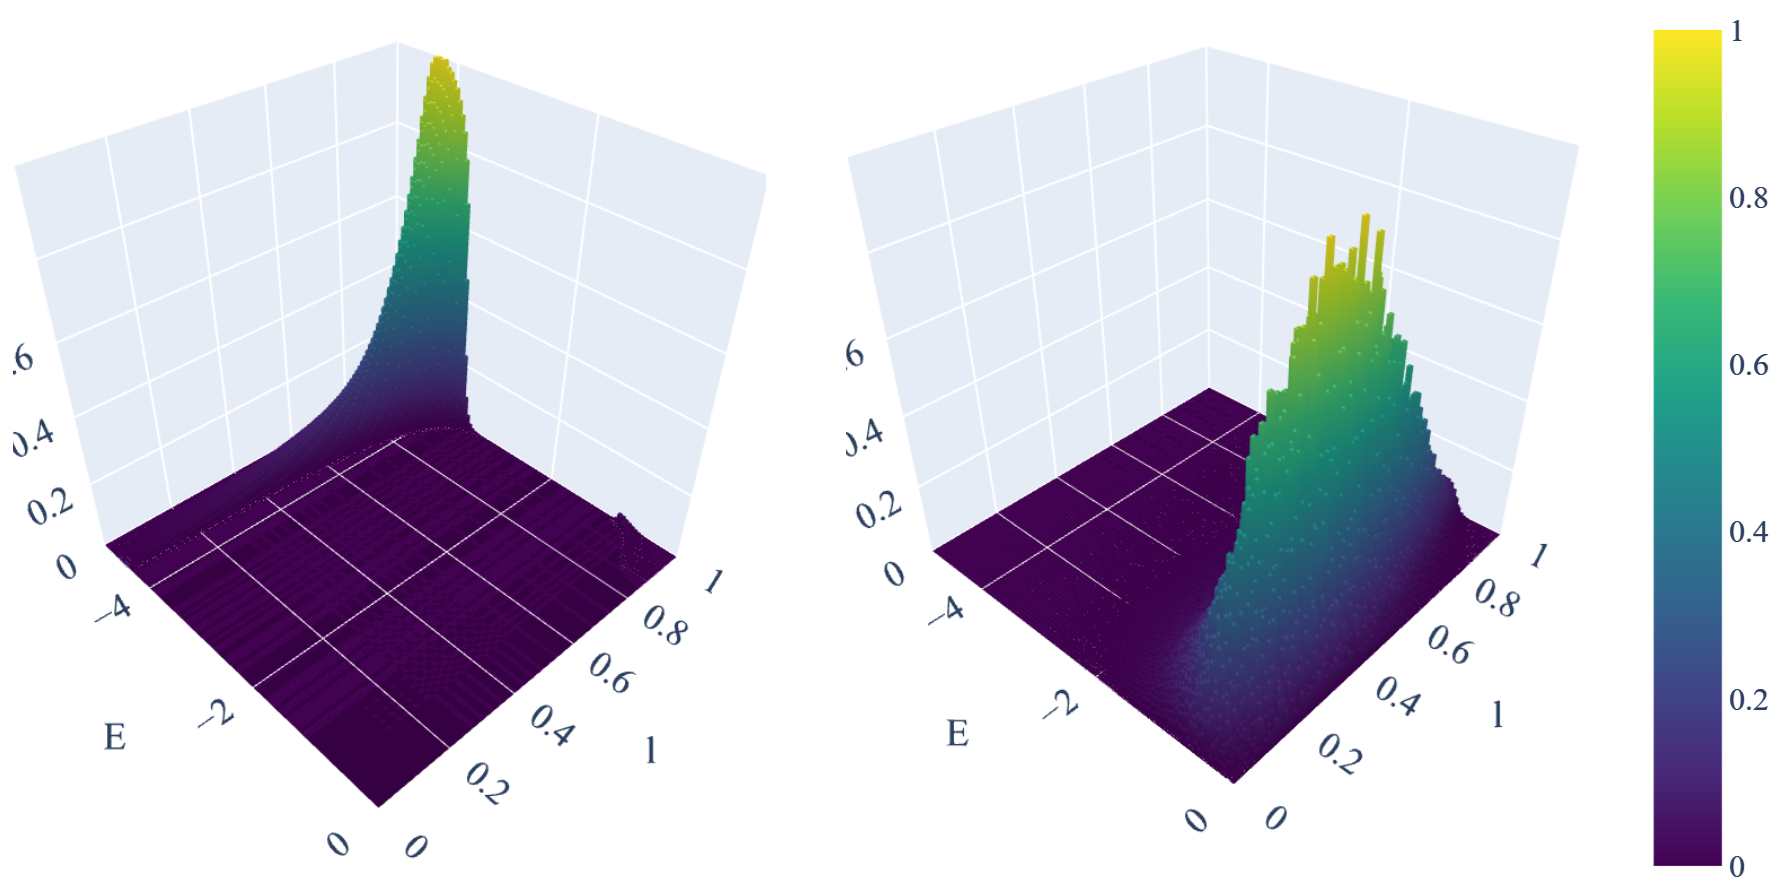
\includegraphics[width=0.7\textwidth]
	{images/Dout100_100.png}
	\caption{Распределение частиц в конце эволюции для $m_{\chi} = 100\, \text{GeV}$, $\delta = 100\, \text{keV}$.}
	\label{fig:Dout100_100}
\end{figure}

\begin{figure}[!h]
\centering
\begin{tikzpicture}
	\begin{axis}[
		%title = {Распределение по $r/R_{\odot}$},
		no markers,
		xmin=0,
		xmax=0.2,
		xtick distance=0.02,
		 xticklabel style={
			/pgf/number format/fixed
		},
		xlabel = \(r\),
		ylabel = {\(\cfrac{d^3N}{d^3r}\)},
		table/col sep = semicolon,
		height = 0.2\paperheight, 
		width = 0.8\paperwidth,
		/pgf/number format/1000 sep={}
		]
		\addplot table [mark=none, x={R}, y={D100}]{tables/CaptDout100_100and50.csv};
		\addplot table [mark=none, x={R}, y={D50}]{tables/CaptDout100_100and50.csv};
		\addplot table [mark=none, x={R}, y={C100}]{tables/CaptDout100_100and50.csv};
		\addplot table [mark=none, x={R}, y={C50}]{tables/CaptDout100_100and50.csv};
		\addplot table [mark=none, x={R}, y={N}]{tables/Term100.csv};
		\legend{ 
			{$N(T_{\odot})$, $\delta = 100\text{keV}$},
			{$N(T_{\odot})$, $\delta = 50\text{keV}$},
			{$C$, $\delta = 100\text{keV}$},
			{$C$, $\delta = 50\text{keV}$},
			{$N_{therm}$}			
		};
	\end{axis}
\end{tikzpicture}
	\caption{Концентраця частиц тёмной материи массы $m_{\chi} = 100\text{GeV}$}
	\label{plot:Nrdistrib}
\end{figure}

Главный вопрос заключается в отношении скорости аннигиляции и скорости захвата $C/A$. Мы рассматриваем уравнение эволюции как с учётом аннигиляции так и без учета аннигиляции. 

\begin{figure}[!h]
	\centering
	\begin{tikzpicture}
		\begin{axis}[
			%title = {Распределение по $r/R_{\odot}$},
			no markers,
			xlabel = {$\delta$, $\text{keV}$},
			ylabel = {Rate, $\frac{1}{\text{s}}$},
			ymode=log,
			table/col sep = semicolon,
			height = 0.2\paperheight, 
			width = 0.8\paperwidth,
			/pgf/number format/1000 sep={}
			]
			\addplot table [mark=none, x={dM}, y={C}]{tables/CaptAnn_noAnn100.csv};
			
			\addplot table [mark=none, x={dM}, y={A}]{tables/CaptAnn_noAnn100.csv};
			
			\addplot table [mark=none, x={dM}, y={A}]{tables/Ann_withAnn100.csv};
			
			\addplot table [mark=none, x={dM}, y={Ath}]{tables/CaptAnn_noAnn100.csv};
			\legend{ 
				{Capture},
				{$A$, linear},
				{$A$, nonlinear},
				{$A = C \th^2{\sqrt{at^2C}}$}
			};
		\end{axis}
	\end{tikzpicture}
	\caption{Зависимость от $\delta$ захвата и аннигиляции при линейной и нелинейной эволюции для $m_{\chi} = 100\text{GeV}$}
	\label{plot:CaptAnn}
\end{figure}

Как можно заметить, если включить в уравнение эволюции аннигиляцию, то результат совпадает с оценкой (\ref{eq:AnnNtherm}). 


При больших $\delta$ уменьшается как величина захвата так и коэффициент аннигиляции. При $\delta$ ниже чем $\delta(m_{\chi})$, наступает термализация в уравнении (\ref{eq:Balance}), т.е. темп аннигиляции равен темпу захвата. Изобразим в плоскости $(m_{\chi} - \delta$ границы областей, при которых наступает или не наступает термализация при разных $\sigma_{\chi p}$. V


\begin{figure}[!h]
	\centering
	\begin{tikzpicture}
		\begin{axis}[
			%title = {Распределение по $r/R_{\odot}$},
			no markers,
			xlabel = {$\delta$, $\text{keV}$},
			ylabel = {M, $\text{GeV}$},
			ymode=log,
			table/col sep = semicolon,
			height = 0.3\paperheight, 
			width = 0.6\paperwidth,
			/pgf/number format/1000 sep={}
			]
			\addplot table [mark=none, x={d_40}, y={M}]{tables/DeltaM_SL.csv};
			\addplot table [mark=none, x={d_41}, y={M}]{tables/DeltaM_SL.csv};
			\addplot table [mark=none, x={d_42}, y={M}]{tables/DeltaM_SL.csv};
			\addplot table [mark=none, x={d_43}, y={M}]{tables/DeltaM_SL.csv};
			\addplot table [mark=none, x={d_44}, y={M}]{tables/DeltaM_SL.csv};
			\legend{ 
				{$\sigma_{\chi p} = 10^{-40}$},
				{$\sigma_{\chi p} = 10^{-41}$},
				{$\sigma_{\chi p} = 10^{-42}$},
				{$\sigma_{\chi p} = 10^{-43}$},
				{$\sigma_{\chi p} = 10^{-44}$}
			};
		\end{axis}
	\end{tikzpicture}
	\caption{}
	\label{plot:MDelta_SL}
\end{figure}



Обозначим величину $1/(aT_{\odot}^2)$ как $С_a(\avarage{\sigma_a v})$. Тогда для того чтобы сдлать ограничения для сечения на протоне $\sigma_{\chi p}$ исходя из ограничения на темп аннигиляции $\Gamma$ нужно решить (\ref{eq:AnnNtherm}) и найти темп захвата.

\begin{equation}
	\cfrac{2\Gamma}{C_a} = 
	F\left(\cfrac{C}{C_a}\right)
\end{equation}

где $F(x) = x\th^2{\sqrt(x)}$. Для оценки с точностью $0.06$ можно использовать $F^{-1}(y) \approx \sqrt{y(1+y)}$.

Тогда, зная $C/C_a$ и $C(\sigma_{\chi p,0})$ --- захват при $\sigma_{\chi p} = \sigma_{\chi p, 0}$ можно найти ограничение для сечения $\sigma_{\chi p}$
\begin{equation}
	\sigma_{\chi p} = \sigma_{\chi p, 0} \cfrac{C_a}{C(\sigma_{\chi p,0})} F^{-1}\left(	\cfrac{2\Gamma}{C_a}\right)
\end{equation}



	
	\section{Summary}
	
	\section{Appendix}
	\subsection{Computational details}
	%	Формула перехода из размерных в безразмерные
%	Формула аннигиляции 
%	Рисунок неравномерной решетки
%	Схема дискретизации по времени
%   Расчет с аннигиляцией
Уравнение термализации (\ref{eq:evolution}) решается в безразмерном виде, где вводится относительное число частиц $\tilde{N}_i = N_i/N_{\odot}$, а также относительное время $\tau = t/T_{\chi p}$.

Уравнение тогда примет вид:
\begin{equation}
	\label{eq:relevolve}
	\deriv{\tilde{N}_i}{\tau} = c_i +
	\sum_j{[s_{ij} \tilde{N}_{j} - s_{ji} \tilde{N}_{i} ]} - e_{i} \tilde{N}_i - a_{\gamma} \sum_j {a_{ij} \tilde{N}_j \tilde{N}_i}
\end{equation}

Для нахождения относительной концентрации $\tilde{n}(r)$ мы считаем сумму интегралов по всем бинам методом Монте-Карло
\begin{equation}
	\label{eq:reldens}
	\tilde{n}(r) = \sum_i{\int{\cfrac{4\pi}{3} \cfrac{1}{2\pi T(E,L)} \cfrac{d\tilde{N}_i}{dEdL^2} dE d\sqrt{v^2-\frac{L^2}{r^2}} }}
\end{equation}

Реальная концентрация тогда равна $n(r) = \tilde{n}(r) n_{\chi 0.4}$. 

Здесь $E$ и $L$ --- энергия и момент импульса согласно (\ref{eq:dimentionless}). 

Матрица аннигилляции $a_{ij}$ из (\ref{eq:evolution}) равна

\begin{equation}
	a_{ij} = \int{3r^2dr \tilde{n}_i(r)\tilde{n}_j(r)}
\end{equation}

где $\tilde{n}_i(r)$ --- относительная концентрация из (\ref{eq:reldens}), посчитанная только для бина $i$.


Для уравнения (\ref{eq:relevolve}) численно мы вводили переменную-вектор $\tilde{C}_{i}$ и решали следующее уравнение:

\begin{equation}
\begin{split}
	\tilde{C}_i = \deriv{\tilde{N}_i}{\tau} \\
	\deriv{\tilde{C}_i}{\tau} = S_{ij} \tilde{C}_{i} - a_{\gamma} [a_{ij} \tilde{N}_i \tilde{C}_{j} - a_{ij} \tilde{N}_j \tilde{C}_{i}] \\
	\tilde{C}_i(0) = c_i
\end{split}
\end{equation}

где матрица $S$ определяется так:
\begin{equation}
	S_{ij} = s_{ij} - \delta_{ij} \sum_{k}{s_{kj}} - \delta_{ij} e_{i}
\end{equation}

Для решения линейной части уравнения мы использовали неявную схему 2 порядка:

\begin{equation}
\begin{split}
	\tilde{C}(\tau + h_{\tau}) = R_L(h_{\tau}) \tilde{C} \\
	R_L(h_{\tau}) = \cfrac{2}{1 - \frac{h_{\tau}}{2}S} - \cfrac{1}{1 - h_{\tau}S}
\end{split}
\end{equation}

Нелинейные эффекты можно оценить схемой 1 порядка:

\begin{equation}
	\begin{split}
		\tilde{C}(\tau + h_{\tau}) = R_{NL}(h_{\tau}) R_L(h_{\tau}) \tilde{C} \\
		[R_{NL}(h_{\tau}) C]_i = e^{-h_{\tau} a_{\gamma} \sum_j{a_{ij}\tilde{N}_j} } (\delta_{ik} - h_{\tau} a_{\gamma} [a_{ik}\tilde{N}_i - \delta_{ik}\sum_{m}{a_{im}\tilde{N}_m}])
		e^{-h_{\tau} a_{\gamma} \sum_j{a_{kj}\tilde{N}_j} } \tilde{C}_k
	\end{split}
\end{equation}





	%\subsection{Verification of results}
	\subsection{Numerical correctness of schemes}
	%	Сходимость схем для упругого случая
%	Сходимость схемы для неупругого случая
%	Собственные значения матрицы рассеяния+ 
%   независимость результатов от шага по времени.

Для проверки точности численных схем, мы рассмотрели эволюцию в упругом и неупругом случае.

В упругом случае мы увеличивали число бинов по энергии и смотрели, как зависит аннигиляция от числа бинов $N_E$ после термализации. 

Хотя наивно схема имеет первый порядок точности, на самом деле порядок может быть и вторым.

Рассмотрим уравнение эволюции:

\begin{equation}
	\deriv{f(X)}{t} = \int{S(X,X')f(X')dX'} - 	 f(X)\int{S(X',X)dX'} 
\end{equation}

Пусть $P_h$ --- проектор решения на сетку. Тогда
\begin{equation}
	P_h\deriv{f(X)}{t} = P_h\int{S(X,X')f(X')dX'} - 	 P_h f(X)\int{S(X',X)dX'} 
\end{equation}

\begin{equation}
	\deriv{f_h(X)}{t} = \mu(dX)^{-1} \int{S(X,X')[f(X')-f(X)]dX'dX}
\end{equation}

После дискретизации оператор эволюции $S$ равен 
\begin{equation}
	S_h(X,X') = \mu(dX)^{-1} \mu(dX')^{-1} \int{S(X,X')dXdX'}
\end{equation}

Положим $S(X,X') = S(X_0,X_0') + A\Delta X + B \Delta X') + O(h^2)$. Из чего следует, что $S_h(X,X')$ = $S(X_0,X_0')$. 

Далее положим, что $f(X) = f_h(X) + F_1\Delta X$

Тогда 

\begin{equation}
	\deriv{f_h(X)}{t} = \mu(dX)^{-1} \int{S_h(X,X')[f_h(X')-f_h(X)]dX'dX} + O(h^2) 
\end{equation}

Получаем, что если $S(X,X')$ и $f(X)$ --- гладкие, то схема имеет 2 порядок точности по $E,L$.



Для проверки сходимости в упругом случае мы нашли конечное распределение частиц тёмной материи при разных шагах решетки и вычислили среднюю энергию и темп аннигиляции на этих распределениях. В упругом случае мы рассматривали зависимость от шага по энергии $h_e$, который мы уменьшали в 2 раза. Поскольку термальное распределение по моменту импульса не зависит от $L$ и схема по $h_L$ не имеет ошибки, мы рассматривали зависимость только от $h_e$. 



\begin{figure}[!h]
	\centering
	\begin{tikzpicture}
		\begin{axis}[
			at={(0,0)}, % Позиция (можно регулировать)
			width=0.5\textwidth,
			height=0.4\textwidth,
			table/col sep = semicolon,
			xmin=0,
			xlabel = { \(h_e/{T_{\odot}} \)},
			ylabel = {\(\avarage{E}/\avarage{E_{1/8}}\)}
			]
			\addplot table [only marks, scatter,x={he}, y={E}]{tables/Conv10.csv};
			\addplot [no marks,domain=0:1.7] {0.999 + 0.02*x^2};
		\end{axis}
		\begin{axis}[
			at={(0.5\textwidth,0)}, % Позиция (можно регулировать)
			width=0.5\textwidth,
			height=0.4\textwidth,
			table/col sep = semicolon,
			xmin=0,
			xlabel = { \(h_e/{T_{\odot}} \)},
			ylabel = {\(A/A_{1/8}\)}
			]
			\addplot table [x={he}, y={A}]{tables/Conv10.csv};
			\addplot [no marks,domain=0:1.7] {1.003 - 0.048*x^2};
		\end{axis}
	\end{tikzpicture}
	\caption{Зависимость средней энергии $\avarage{E}$ и аннигиляции $A$ при $m = 10 \text{GeV}$. Шаг по энергии указан в единицах температуры Солнца в центре $T_{\odot}$. Значения нормированны на значениях при минимальном шаге.}
	\label{plot:ConvEl10}
\end{figure}

В неупругом случае мы рассматривали сетки с разбиением по $E$ и $l$ на $50$,$100$ и $200$ равномерных отрезков.
Величина аннигиляции почти не зависела от $h_e$ и демонстрировала линейную сходимость по $h_l$




\begin{figure}[!h]
	\centering
	\begin{tikzpicture}
		\begin{axis}[
			at={(0,0)}, % Позиция (можно регулировать)
			width=0.5\textwidth,
			height=0.4\textwidth,
			table/col sep = semicolon,
			xmin=0,
			xlabel = { \(h_e (1 = E_{max}/50) \)},
			ylabel = {\(A/A_{1/4,1/4}\)},
			legend style={
				at = {(0.3,0.8)},
				anchor=north
			}
			]
			\addplot table [x={h}, y={nl0}]{tables/ConvInel_E.csv};
			\addplot table [x={h}, y={nl1}]{tables/ConvInel_E.csv};
			\addplot table [x={h}, y={nl2}]{tables/ConvInel_E.csv};
			\legend{ 
				{$h_l = 1\ \ \ $},
				{$h_l = 1/2$},
				{$h_l = 1/4$}
			};
		\end{axis}
		\begin{axis}[
			at={(0.5\textwidth,0)}, % Позиция (можно регулировать)
			width=0.5\textwidth,
			height=0.4\textwidth,
			table/col sep = semicolon,
			xmin=0,
			xlabel = { \(h_l (1 = L_{max}/50) \)},
			ylabel = {\(A/A_{1/4,1/4}\)},
			legend style={
				at = {(0.2,0.98)},
				anchor=north
			}
			]
			\addplot table [x={h}, y={ne0}]{tables/ConvInel_L.csv};
			\addplot table [x={h}, y={ne1}]{tables/ConvInel_L.csv};
			\addplot table [x={h}, y={ne2}]{tables/ConvInel_L.csv};
			\legend{ 
				{$h_e = 1\ \ \ $},
				{$h_e = 1/2$},
				{$h_e = 1/4$}
			};
		\end{axis}
	\end{tikzpicture}
	\caption{Зависимость средней энергии $\avarage{E}$ и аннигиляции $A$ при $m = 10 \text{GeV}$. Шаг по энергии указан в единицах температуры Солнца в центре $T_{\odot}$. Значения нормированны на значениях при минимальном шаге. $m_{\chi} = 100 \text{GeV}$, $\delta= 100 \text{keV}$}
	\label{plot:ConvInel100}
\end{figure}


	
	\section{Bibliography}
	
	
\end{document}